\documentclass[12pt,a4paper]{article}
\usepackage[UTF8]{ctex}
\usepackage{graphicx}
\usepackage{geometry}
\usepackage{ulem}
\usepackage{enumitem}
\usepackage{titlesec}
\usepackage{multicol}
\usepackage[export]{adjustbox}
\usepackage{amsmath}  % 推荐用于更好的数学排版
\usepackage[utf8]{inputenc}
\usepackage{CJKutf8}
\usepackage{fancyhdr}
\usepackage{lastpage}
\usepackage{ulem}
\usepackage{tabularx}
\usepackage{float}

% 页眉页脚设置
\pagestyle{fancy}
\fancyhf{} % 清除所有页眉页脚
% 设置页眉内容
%-==========1. 填写从第二页开始 每页第一行的信息==========-
\fancyhead[C]{
    \makebox[4.5em][c]{实验名称：} \uline{\makebox[14em][c]{OrCAD软件使用练习}} 
    \makebox[2.5em][c]{姓名：} \uline{\makebox[4em][c]{}} 
    \makebox[2.5em][c]{学号：} \uline{\makebox[5em][c]{}}
}%--------------------------------------------------------
\fancyfoot[C]{第 \thepage\ 页，共 \pageref{LastPage} 页}

% 取消页眉和页脚的下划线
\renewcommand{\headrulewidth}{0pt} % 页眉横线粗细设为0
\renewcommand{\footrulewidth}{0pt} % 页脚横线粗细设为0

% 调整页眉高度
\setlength{\headheight}{50pt}

% 设置plain样式（用于第一页）
\fancypagestyle{plain}{
    \fancyhf{} % 清除所有页眉页脚
    \renewcommand{\headrulewidth}{0pt} % 隐藏页眉横线
    \fancyfoot[C]{第 \thepage\ 页，共 \pageref{LastPage} 页} % 保留页脚
}
% 设置页面边距
\geometry{left=2.54cm,right=1.5cm,top=2.54cm,bottom=2.54cm}

% 设置正文字体大小为小四
\renewcommand{\normalsize}{\fontsize{12pt}{16pt}\selectfont}
% 设置章节格式
\titleformat{\section}{\fontsize{16pt}{22pt}\selectfont\bfseries}{\thesection}{1em}{} % 一级标题：三号
\titleformat{\subsection}{\fontsize{15pt}{20pt}\selectfont\bfseries}{\thesubsection}{1em}{} % 二级标题：小三

\begin{document}
\thispagestyle{plain}%第一页使用 plain 样式，而不是默认的 fancy 样式，第一页不再显示页眉
% 标题部分 - 两栏布局
\begin{multicols}{2}
    % 左栏：图片和实验报告标题
    % 左栏：使用空行创建前三行
    \noindent
    ~\\ % 第一行
    ~\\ % 第二行
    ~\\ % 第三行
    \hphantom{占位}% 使用空占位符
    \raisebox{-0.5\baselineskip}% 图片向下移动半行
    {
\includegraphics[width=1.85in,height=0.58in]{ZJU.jpg}}
    \hspace{.5em}% 图片和标题之间的间距
    \raisebox{0pt}[\height][0pt]% 标题底部对齐
    {\textbf{\fontsize{26pt}{30pt}\selectfont 实验报告}}
    
    \columnbreak % 换到右栏
    
    % 右栏：个人信息
    % 右栏：个人信息 - 靠右对齐 
%-==========2. 填写个人信息==========-
    \begin{flushright}
        \makebox[3em][l]{专业：} \uline{\makebox[9em][c]{法语-电子科学与技术}} \\
        \makebox[3em][l]{姓名：} \uline{\makebox[9em][c]{}} \\
        \makebox[3em][l]{学号：} \uline{\makebox[9em][c]{}} \\
        \makebox[3em][l]{日期：} \uline{\makebox[9em][c]{2025年11月25日}} \\
        \makebox[3em][l]{地点：} \uline{\makebox[9em][c]{紫金港东四216}} \\
    \end{flushright}   
\end{multicols}
% 课程名称等信息（单栏）
%-==========3. 填写课程信息==========-
\noindent
课程名称： \uline{电子电路设计实验I} \hfill 指导老师： \uline{施红军、叶险峰、邓靖靖} \hfill 成绩： \uline{\hspace{3cm}} \\
实验名称： \uline{OrCAD软件使用练习} \hfill 实验类型： \uline{验证实验} \hfill 同组学生姓名： \uline{}
%-==========4. 正文开始==========-
\section*{一、实验目的}

1、了解 OrCAD 套件中的 Capture 和 PSpice A/D 软件的常用菜单和命令的使用。

2、掌握 OrCAD 中 Capture 软件的电路图输入和编辑方法。

3、学习 OrCAD 中 PSpice A/D 软件的分析设置、仿真、波形查看的方法。

4、学习半导体器件特性、电路特性的仿真分析方法。

\section*{二、实验任务与要求}

1、二极管特性的仿真分析 （讲义P86-89）

\begin{figure}[H]
    \centering
    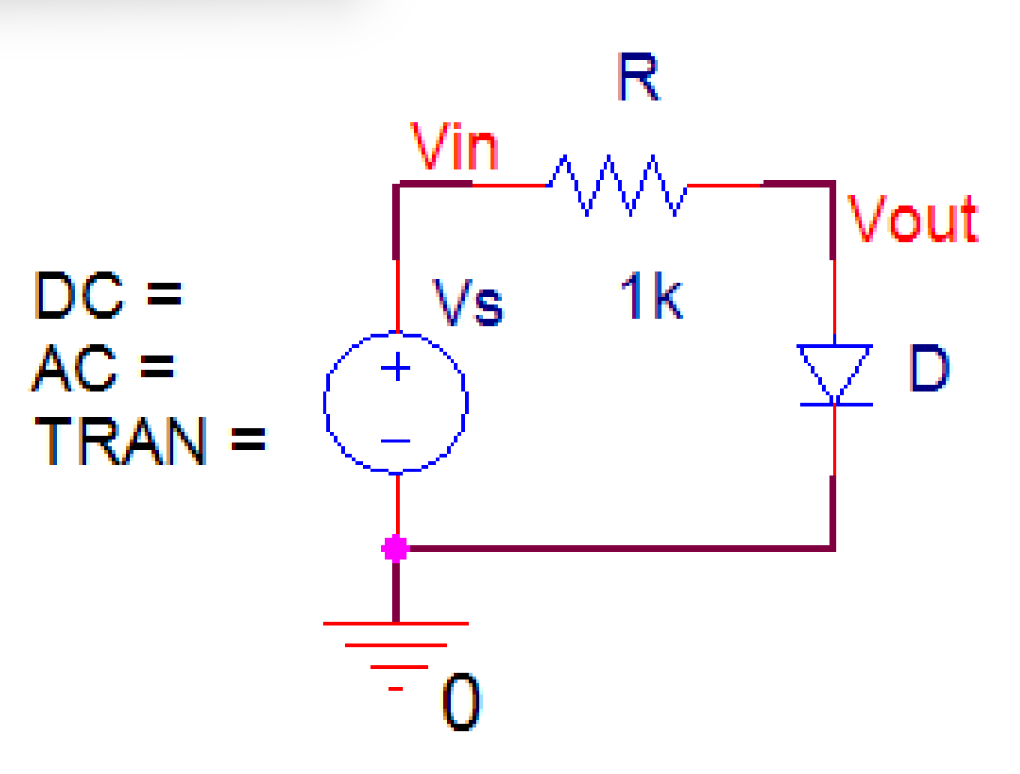
\includegraphics[width=0.3\textwidth, height=0.15\textheight]{0.png}
    \caption{二极管特性测试电路}
    \label{fig0}
\end{figure}


2、桥式整流电路的瞬态分析：查看输出波形情况。

\begin{figure}[H]
    \centering
    
\includegraphics[width=0.25\textwidth, height=0.1\textheight]{1.png}
    \caption{桥式整流电路}
    \label{fig1}
\end{figure}

3、稳压二极管电路的瞬态分析：当采用50Hz、9V正弦电压源Vi，交流电压信号经过两个对头放置的稳压二极管后的输出波形情况。

\begin{figure}[H]
    \centering
    
\includegraphics[width=0.4\textwidth, height=0.2\textheight]{2.png}
    \caption{稳压二极管电路}
    \label{fig2}
\end{figure}



\section*{三、实验步骤}

\subsection*{1、二极管特性的仿真分析}

\subsubsection*{(1)、绘制电路图}
从元件库中依次取出 VSRC、R、D1N4148、AGND 等元件放置在电路图上，并进行连线。将电阻的阻值设为 1kΩ，电阻名称设为 R，电压源名称设为 \(V_s\)，电路图连接如下：

\begin{figure}[H]
    \centering
    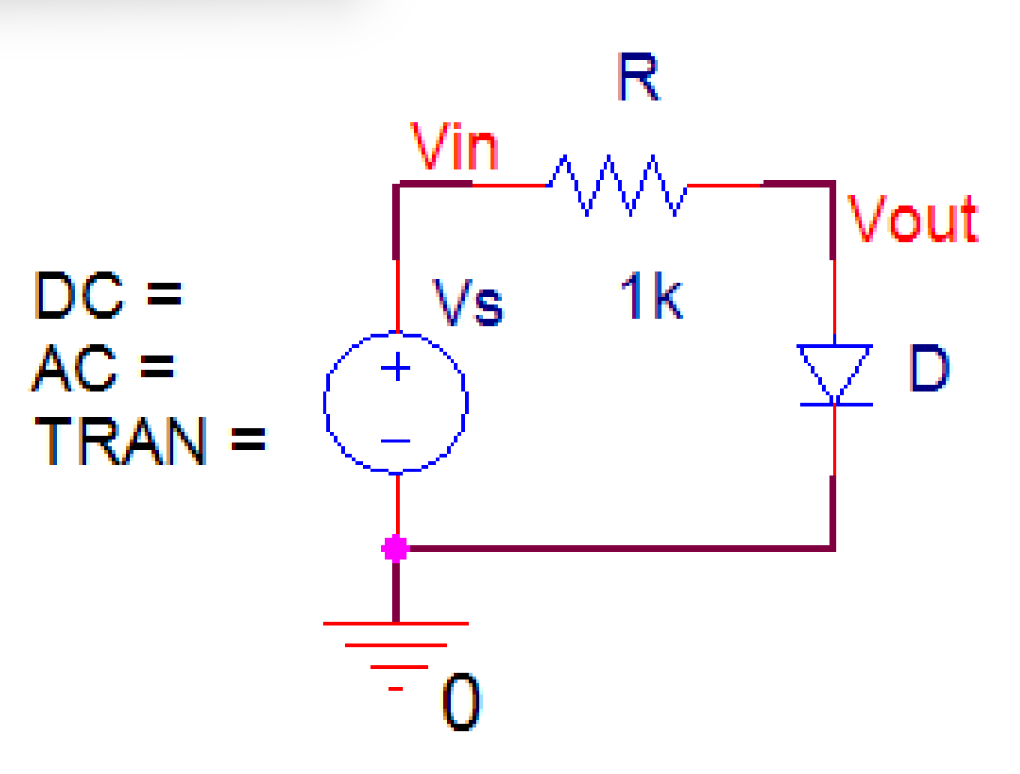
\includegraphics[width=0.3\textwidth, height=0.15\textheight]{0.png}
    \caption{二极管仿真电路}
    \label{fig3}
\end{figure}


\subsubsection*{(2)、设置分析参数}
为了仿真分析二极管的伏安特性，需要对电压源Vs进行直流扫描（DC Sweep）分析。

为了仿真二极管的正向导通特性、反向特性和击穿特性，应使Vs的变化范围足够大。所以，二极管测试电路的直流扫描分析参数可设置为：扫描变量类型为电压源，扫描变量为Vs，扫描类型为线性扫描，初始值为-200V，终值为40V，增量为0.1V。

\begin{figure}[H]
    \centering
    
\includegraphics[width=0.5\textwidth, height=0.3\textheight]{4.png}
    \caption{设置直流扫描分析参数}
    \label{fig4}
\end{figure}


为了仿真分析二极管在不同温度下的伏安特性，同时设置直流扫描的次要分析。设置扫描变量类型为温度，扫描类型为列表扫描，扫描值为-10（℃），0（℃），30（℃），如下：

\begin{figure}[H]
    \centering
    
\includegraphics[width=0.5\textwidth, height=0.3\textheight]{5.png}
    \caption{设置直流扫描次要分析参数}
    \label{fig5}
\end{figure}

\subsubsection*{(3) 运行仿真分析程序}
在 Capture 程序中按 F11 功能键或从 PSpice 主菜单中选择
Run 命令，调出 PSpice A/D 程序对所输入的二极管特性测试电路进行直流扫描仿真分析。

先显示 \(I(D)\) 曲线。该曲线只是二极管电流与电压源之间的关系，还不是二极管的伏安特性曲线。

\begin{figure}[H]
    \centering
    
\includegraphics[width=0.8\textwidth, height=0.3\textheight]{6.png}
    \caption{二极管电流与电压源之间的关系}
    \label{fig6}
\end{figure}


为了得到二极管的伏安特性曲线，将横坐标变量改为二极管两端的电压，选择二极管电压V(D:1)作为X。得到如下波形：

\begin{figure}[H]
    \centering
    
\includegraphics[width=0.8\textwidth, height=0.3\textheight]{7.png}
    \caption{二极管的伏安特性曲线}
    \label{fig7}
\end{figure}

从图中可以看出二极管正偏时导通，电压近似为0；二极管反偏时截止，电流近似为0；当反向偏置电压过大时，则二极管处于反向击穿状态，反向电流将急剧增大。

\subsubsection*{(4) 二极管在不同温度下的正向伏安特性曲线}
为了得到二极管在不同温度下的正向伏安特性曲线，需改变X轴和Y轴的坐标范围。将X轴坐标范围设置为0V至1V，将Y轴坐标范围设置为0mA至40mA。

得到的不同温度下的特性曲线如图\ref{fig8}所示。

\begin{figure}[H]
    \centering
    
\includegraphics[width=0.8\textwidth, height=0.3\textheight]{8.png}
    \caption{二极管在不同温度下的正向伏安特性曲线}
    \label{fig8}
\end{figure}


最左边的特性曲线为30℃时的伏安特性，中间曲线是0℃时的伏安特性，右边曲线是-10℃时的伏安特性，温度升高时二极管电流增大。且能够发现30℃时的伏安特性曲线与0℃时的伏安特性曲线之间的间隔要比0℃时的伏安特性曲线与-10℃时的伏安特性曲线的间隔大。

\subsubsection*{(5) 仿真二极管两端的电压波形}
为了仿真分析二极管两端的电压波形，需要在电路中加入瞬态电源。

将电路中的电源Vs用VSIN元件代替，并设置元件参数为VOFF=0，VAMPL=10V，FREQ=1kHz。并且，根据电源的特性，设置参数 Run to time=2ms，Maximum step size=0.01ms，最终得到的二极管波形如图\ref{fig9}所示。

\begin{figure}[H]
    \centering
    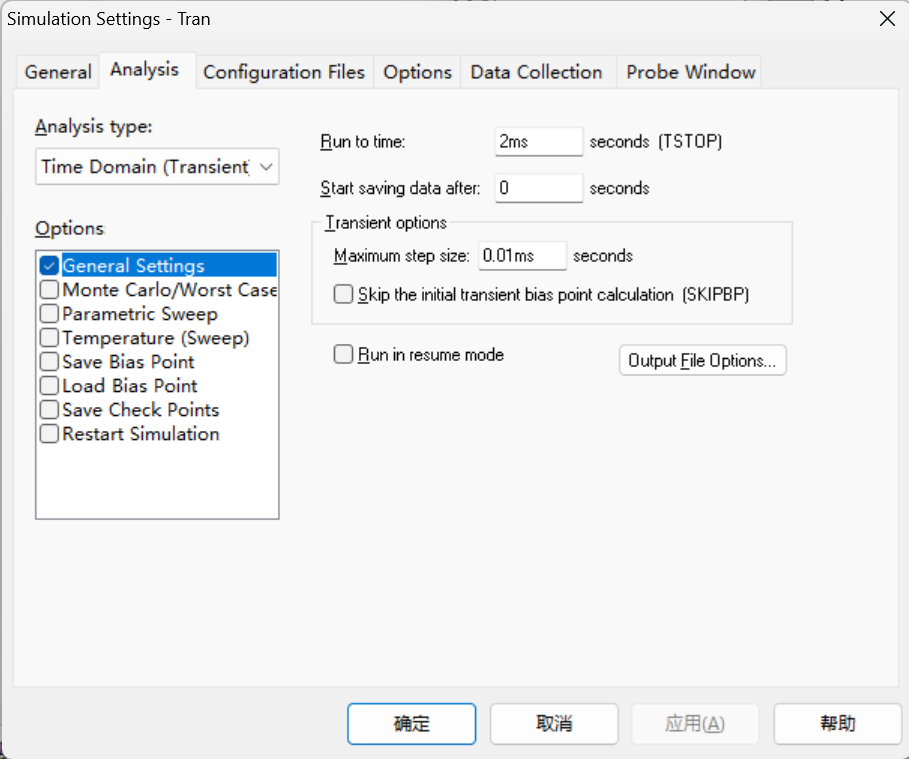
\includegraphics[width=0.5\textwidth, height=0.3\textheight]{20.png}
    \caption{设置分析参数}
    \label{fig20}
\end{figure}

\begin{figure}[H]
    \centering
    
\includegraphics[width=0.8\textwidth, height=0.3\textheight]{9.png}
    \caption{二极管两端的电压波形}
    \label{fig9}
\end{figure}

\section*{2、桥式整流电路瞬态分析}

\subsubsection*{(1) 实验电路绘制}
实验给出的理论电路图如图\ref{fig1}所示。按照要求进行绘制，其中令 \( R \) 的一侧接地，另一侧作为测试点\( V_o \) 进行电压测量。

\begin{figure}[H]
    \centering
    
\includegraphics[width=0.6\textwidth, height=0.2\textheight]{10.png}
    \caption{仿真电路图}
    \label{fig10}
\end{figure}

\subsubsection*{(2) 电压源设置}
电压源 VSIN 使用正弦输入，设置为 50Hz, 12V。

\subsubsection*{(3) 扫描参数设置}
由于电压源频率为50Hz, 设置 Run to time 为两个周期即 0.04s, maximum step size 为 2ms:

\begin{figure}[H]
    \centering
    
\includegraphics[width=0.5\textwidth, height=0.3\textheight]{11.png}
    \caption{设置扫描分析参数}
    \label{fig11}
\end{figure}

\subsubsection*{(4) 运行仿真}

运行仿真，得到如下输出波形：

\begin{figure}[H]
    \centering
    
\includegraphics[width=0.8\textwidth, height=0.3\textheight]{12.png}
    \caption{仿真波形}
    \label{fig12}
\end{figure}

如图\ref{fig12}所示，输出电压的幅度和输入电压的幅度相差约为2倍的$V_D$，即
$$V_o-V_s=2V_D$$
和理论相符合，说明该桥式整流二极管起到了整流的作用。

\section*{3、稳压二极管电路瞬态分析}

\subsubsection*{(1) 电压源设置}
电压源 VSIN 使用正弦输入，设置为 50Hz，9V。

\subsubsection*{(2) 绘制电路图}
实验理论图如\ref{fig2}所示，为了显示稳压二极管对于电压的影响，我们测量两个点的电压，绘制的电路图如图所示：

\begin{figure}[H]
    \centering
    
\includegraphics[width=0.6\textwidth, height=0.2\textheight]{13.png}
    \caption{仿真电路图}
    \label{fig13}
\end{figure}

\subsubsection*{(3) 查看稳压二极管参数}
利用 Edit PSpice Model 查看其各项参数值，稳压值即 $B_V=4.7\mathrm{V}$。

\begin{figure}[H]
    \centering
    
\includegraphics[width=1\textwidth, height=0.15\textheight]{14.png}
    \caption{Edit PSpice Model中的各项参数值}
    \label{fig14}
\end{figure}


\subsubsection*{(4) 扫描参数设置}
由于电压源频率仍为50Hz，仍设置Run to time为两个周期即0.04s, maximum step size为2ms。


\begin{figure}[H]
    \centering
    
\includegraphics[width=0.5\textwidth, height=0.3\textheight]{11.png}
    \caption{设置扫描分析参数}
    \label{fig11b}
\end{figure}

\subsubsection*{(5) 运行仿真}
运行仿真，实验波形如图所示。可以发现，相较于电压源两端的值，R两端的电压被钳制在了一个范围内。

\begin{figure}[H]
    \centering
    
\includegraphics[width=0.8\textwidth, height=0.3\textheight]{15.png}
    \caption{仿真波形}
    \label{fig15}
\end{figure}

\subsubsection*{(6) 利用cursor测量稳压二极管两端电压\(V_o\)的峰值}
可以发现电压值约为稳压二极管的稳压值，即4.7V。

\begin{figure}[H]
    \centering
    
\includegraphics[width=1\textwidth, height=0.15\textheight]{16.png}
    \caption{利用cursor测量稳压二极管两端电压\(V_o\)的峰值}
    \label{fig16}
\end{figure}

\section*{四、心得与体会}

本次实验使我对ORCAD软件的操作有了系统性掌握，从电路绘制、仿真参数设置到波形分析，完成了完整的仿真流程。

通过仿真，我直观地验证了二极管的单向导电性、反向击穿等特性，并观察到温度对其特性的显著影响。在桥式整流和稳压电路实验中，我进一步理解了二极管在实际电路中的应用价值。

此次实验让我认识到电路仿真作为理论联系实际的重要桥梁，不仅能深化对知识的理解，也极大地提升了工程实践能力。

\end{document}